\section{Produktdaten}

%\comment{Was speichert das Produkt (langfristig) aus Benutzersicht?}

\begin{description}
  \item[/D010/]
    \textit{Automatendefinition:} Die Struktur eines endlichen Automaten, bestehend aus Zust�nden und �bergangen, wird in einer XML-Datei gespeichert, die der folgenden Definition (Listing \ref{xsd}) gen�gt.
    
    \lstset{ %
  language=XML,                % the language of the code
  basicstyle=\footnotesize,           % the size of the fonts that are used for the code
  numbers=left,                   % where to put the line-numbers
  numberstyle=\footnotesize,          % the size of the fonts that are used for the line-numbers
  stepnumber=2,                   % the step between two line-numbers. If it's 1, each line 
                                  % will be numbered
  numbersep=5pt,                  % how far the line-numbers are from the code
  backgroundcolor=\color{white},      % choose the background color. You must add \usepackage{color}
  showspaces=false,               % show spaces adding particular underscores
  showstringspaces=false,         % underline spaces within strings
  showtabs=false,                 % show tabs within strings adding particular underscores
  frame=single,                   % adds a frame around the code
  tabsize=2,                      % sets default tabsize to 2 spaces
  captionpos=b,                   % sets the caption-position to bottom
  breaklines=true,                % sets automatic line breaking
  breakatwhitespace=false,        % sets if automatic breaks should only happen at whitespace
  title=\lstname,                   % show the filename of files included with \lstinputlisting;
                                  % also try caption instead of title
  numberstyle=\tiny,        % line number style
  escapeinside={\%*}{*)},            % if you want to add a comment within your code
  morekeywords={*,...}               % if you want to add more keywords to the set
}

\begin{lstlisting}[caption=XSD,label=xsd]
<?xml version="1.0" encoding="UTF-8"?>
<xs:schema xmlns:xs="http://www.w3.org/2001/XMLSchema"
    elementFormDefault="qualified">

  <xs:element name="finitestatemachine">
    <xs:complexType>
      <xs:sequence>
        <xs:element ref="initialstate"/>
        <xs:element ref="finalstates"/>
        <xs:element ref="transitions"/>
      </xs:sequence>
      <xs:attribute name="name" type="xs:normalizedString"/>
    </xs:complexType>
  </xs:element>

  <xs:element name="initialstate" type="xs:normalizedString"/>

  <xs:element name="finalstates">
    <xs:complexType>
      <xs:sequence>
        <xs:element maxOccurs="unbounded" ref="finalstate"/>
      </xs:sequence>
    </xs:complexType>
  </xs:element>

  <xs:element name="finalstate" type="xs:normalizedString"/>

  <xs:element name="transitions">
    <xs:complexType>
      <xs:sequence>
        <xs:element maxOccurs="unbounded" ref="transition"/>
      </xs:sequence>
    </xs:complexType>
  </xs:element>

  <xs:element name="transition">
    <xs:complexType>
      <xs:sequence>
        <xs:element ref="start"/>
        <xs:element ref="input"/>
        <xs:element ref="ends"/>
      </xs:sequence>
    </xs:complexType>
  </xs:element>

  <xs:element name="start" type="xs:normalizedString"/>

  <xs:element name="input" type="xs:normalizedString"/>

  <xs:element name="ends">
    <xs:complexType>
      <xs:sequence>
        <xs:element maxOccurs="unbounded" ref="end"/>
      </xs:sequence>
    </xs:complexType>
  </xs:element>

  <xs:element name="end" type="xs:normalizedString"/>

</xs:schema>
\end{lstlisting}

	Im Nachfolgenden sind ein beispielhafter Automat (Abbildung \ref{example_automaton}) und die hierzu erzeugte XML-Datei (Listing \ref{example_xml}) aufgef�hrt.

\begin{figure}[h!]
	\centering
	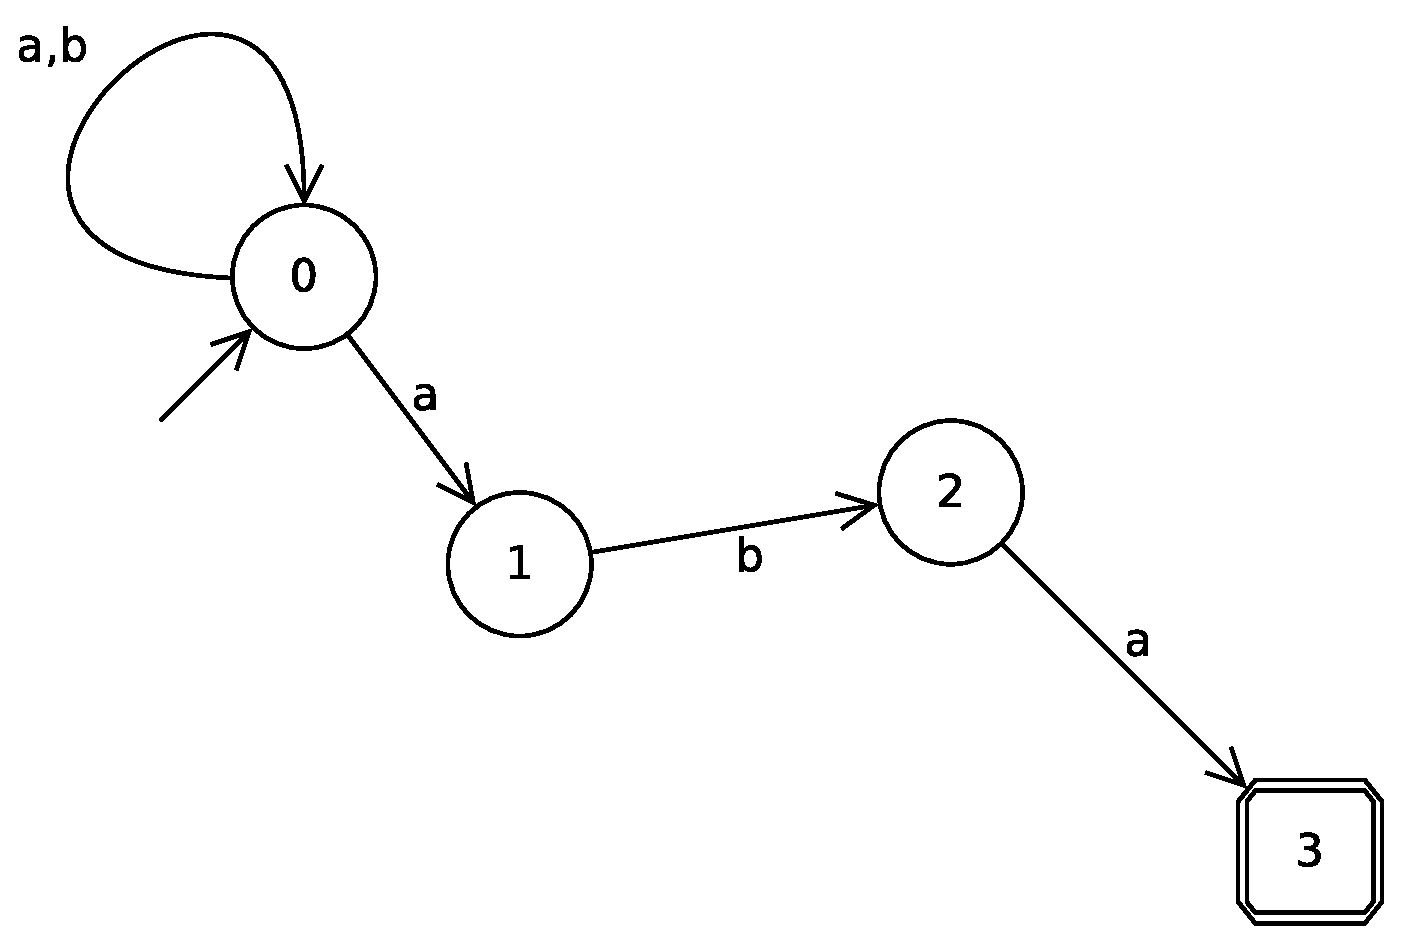
\includegraphics[width=8cm]{images/NFA-1.eps}
	\caption{Ein beispielhafter Automat}
	\label{example_automaton}
\end{figure}

\begin{lstlisting}[caption=Erzeugte XML-Datei,label=example_xml]
<?xml version="1.0" encoding="utf-8"?>
<!DOCTYPE finitestatemachine PUBLIC
  "http://github.com/downloads/wookietreiber
         /scalomator/FiniteStateMachine.dtd">
<finitestatemachine
  xmlns:xsi="http://www.w3.org/2001/XMLSchema-instance"
  xsi:noNamespaceSchemaLocation=
  "http://github.com/downloads/wookietreiber
         /scalomator/FiniteStateMachine.xsd"
  name="foo-o-mat">

  <initialstate>0</initialstate>

  <finalstates>
    <finalstate>3</finalstate>
  </finalstates>

  <transitions>
    <transition>
      <start>0</start>
      <input>a</input>
      <ends>
        <end>0</end>
        <end>1</end>
      </ends>
    </transition>
    <transition>
      <start>0</start>
      <input>b</input>
      <ends>
        <end>0</end>
      </ends>
    </transition>
    <transition>
      <start>1</start>
      <input>b</input>
      <ends>
        <end>2</end>
      </ends>
    </transition>
    <transition>
      <start>2</start>
      <input>a</input>
      <ends>
        <end>3</end>
      </ends>
    </transition>
  </transitions>

</finitestatemachine>

\end{lstlisting}

\end{description}

